\chapter{Riconcilazione sorgenti}

Nel seguito verranno documentati i passi intrapresi nella progettazione
del modello riconciliato o Operational Data Store partendo dalle sorgenti
operazionali descritte nel capitolo precedente.

\section{Ispezione e normalizzazione}

\subsection{Helbiz}

Il livello di granularità delle profilazioni della sorgente Helbiz è
risultato essere troppo basso rispetto alle interrogazioni a cui il data
warehouse si prefigge di rispondere. Inoltre attributi come
\textit{latitude}, \textit{longitude}, \textit{battery\_level\_miles},
\textit{power} e \textit{miles\_range} non si prestano, in quanto valori
numerici continui, ad essere utilizzati all'interno del costrutto di
selezione di una interrogazione OLAP per il dominio applicativo
scelto. Inoltre gli attributi \textit{battery\_level\_miles} e
\textit{miles} risultano essere ridondanti.

Partendo dallo schema ER mostrato in figura~\ref{fig:vehicle_profiling_er} è
stato ricavato lo schema concettuale di figura
\ref{fig:vehicle_interval_profiling_er}.

\begin{figure}[H]                                                                                                                                                            
\centering                                                                                                                                                                   
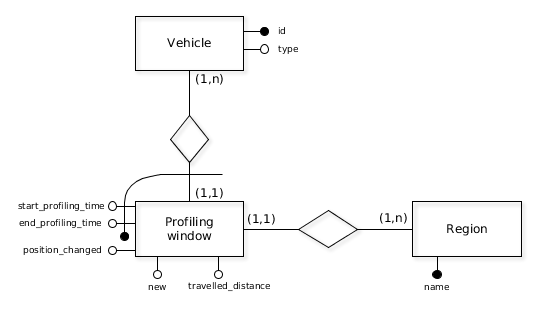
\includegraphics[width=\textwidth]{diagrams/vehicle_interval_profiling_er}                                                                                                                                   
\caption{Diagramma ER Vehicle-Profiling window-Region}                                                                                                                                            
\label{fig:vehicle_interval_profiling_er}                                                                                                                                                           
\end{figure}

Non essendo il nuovo schema una semplice ristrutturazione dello
schema logico di partenza ma un nuovo schema a se stante, l'entità
\textit{Profiling} è stata sostituita con l'entità \textit{Profiling
window}, le cui istanze si riferiscono ai dati profilati all'interno di
un delimitato intervallo di tempo per un determinato veicolo.
Nello specifico sono stati aggiunti i seguenti nuovi attirbuti:
\begin{itemize}
\item \textit{start\_profiling\_time:} istante di inizio della finestra
temporale;
\item \textit{end\_profiling\_time:} istante di fine della finestra temporale;
\item \textit{position\_changed:} attributo che indica se la posizione
del veicolo è variata durante l'intervallo in oggetto;
\item \textit{new:} attributo che indica se un veicolo non presente durante
all'istante di inizio della finestra temporale è stato invece censito
all'istante che delimita la fine della finestra temporale;
\item \textit{travelled\_distance:} attributo che contiene la distanza 
percorsa dal veicolo nella finestra temporale.
\end{itemize}

\noindent~L'attributo \textit{travelled\_distance} corrisponde alla distanza in linea
d'aria tra le coordinate cartesiane della profilazione effettuata all'istante
\textit{start\_profiling\_time} e quella effettuata all'istante
\textit{end\_profiling\_time}.
L'aggiunta dell'attributo \textit{new} è volta a gestire il caso in cui un
veicolo sia stato oggetto di utilizzo ininterrotto da parte di un utente per
un tempo superiore all'intervallo tra due successive profilazioni o il caso in
cui un veicolo sia stato intenzionalmente posizionato in un punto da un addetto
della manutenzione di Helbiz dopo essere stato ricaricato o allo scopo di
redistribuzione la flotta di veicoli a disposizione all'interno della region.
L'attributo \textit{psotion\_changed} è stato aggiunto allo scopo di permettere
una veloce selezione delle istanze dell'entitò in oggetto per le quali lo
spostamento memorizzato nell'attributo \textit{travelled\_distance} risulta essere
maggiore una certa soglia. Come sarà descritto nella parte dedicata alle attività di
ETL eseguite dalle sorgenti operazionali all'ODS, tale attributo permette di
escludere una serie di falsi positivi dati dalla presenza dei veicoli in ambienti
aperti, soggetti agli eventi atmosferici oltre che all'interazione con attori
che si trovano nelle immediate vicinanze.
Inoltre si ha che gli attributi \textit{start\_profiling\_time} e
\textit{end\_profiling\_time} insieme con l'attributo \textit{id} dell'entità
\textit{Vehicle}, identificano univocamente una finestra di profilazione.

Anche quest'ultimo schema risulta lontano dal poter essere integrato con le altre
sorgenti, aventi un livello di granularità temporale minimo di un ora.
Inoltre gli attirbuti \textit{position\_changed} e \textit{new} non sono
sfruttabili in nessuna delle interrogazione derivate dal fatto definito.
Pertanto, partendo dallo schema concettuale di
figura~\ref{fig:vehicle_interval_profiling_er} si è giunti allo schema di figura
\ref{fig:vehcile_hourly_profiling_er}.

\begin{figure}[H]                                                                                                                                                            
\centering                                                                                                                                                                   
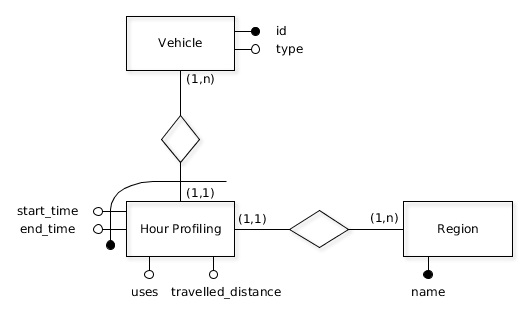
\includegraphics[width=\textwidth]{diagrams/vehicle_hour_profiling_er}                                                                                                                                   
\caption{Diagramma ER Vehicle-Profiling window-Region}                                                                                                                                            
\label{fig:vehicle_hour_profiling_er}                                                                                                                                                           
\end{figure}

Il processo di ristrutturazione ha consistito nella sostituzione dell'entità
\textit{Profiling window} con l'entità \textit{Hourly Profiling} avente i
seguenti nuovi attributi:
\begin{itemize}
\item \textit{start\_time:} istanze d'inzio della finestra di profilazione;
\item \textit{end\_time:} istanze di fine della finestra di profilazione;
\item \textit{uses:} attributo contenente il numero di utilizzi di un
veicolo all'interno della finestra di profilazione;
\item \textit{travelled\_distance:} attributo che contiene la distanza 
percorsa dal veicolo nella finestra di profilazione.
\end{itemize}
Tale schema è pertanto da considerarsi quale schema concettuale definitivo per la
sorgente Helbiz e come uno degli schemi oggetto del sucessivo processo di
integrazione.

\subsection{Torino Meteo}

Similmente a quanto fatto per Helbiz, anche per la sorgente Torino Meteo è
stato necessario modificare lo schema concettuale presentato in figura
\ref{fig:weather_detection_er}. Le profilazioni acquisite dai sensori
sono relative ad un determinato istante di tempo e non ad una finestra temporale
come nel caso di Helbiz e riportano per gli attributi \textit{rain},
\textit{wind}, \textit{relative\_humidity} e \textit{temperature} valori numerici
continui che non si prestano ad essere utilizzati all'interno di un'interrogazione
OLAP quali quelle definite. Inoltre, gli attributi \textit{id} e
\textit{relative\_humidity} non sono di interesse ai fini del progetto.
Lo schema derivato di figura \ref{fig:wheathre_hourly_profiling_er} contiene la
nuova entità \textit{Weather hourly profiling} caratterizzata dai seguenti attributi:
\begin{itemize}
\item \textit{start\_profiling\_time:} istante di inizio dell'intervallo orario in cui
si collocano l'entità in oggetto;
\item \textit{end\_profiling\_time:} ora di fine dell'intervallo orario in cui si
collocano le profilazioni rappresentate dall'entità in oggetto;
\item \textit{rain\_level:} attributo contenente il livello di intensità delle
precipitazioni rilevanto nell'intervallo orario;
\item \textit{wind\_level:} attributo contenente il livello di intensità del
vento rilevato nell'intervallo orario;
\item \textit{temperature\_level:} attributo contenente il livello di intensità della
temperatura rilavato nell'intervallo orario.
\end{itemize}

\begin{figure}[H]                                                                                                                                                            
\centering                                                                                                                                                                   
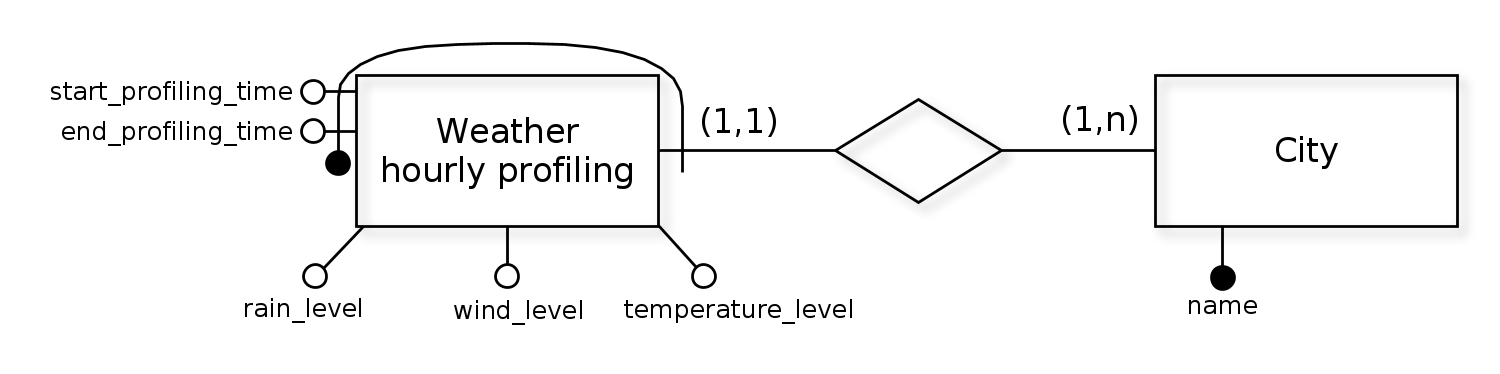
\includegraphics[width=\textwidth]{diagrams/wheathre_hourly_profiling_er}                                                                                                                                   
\caption{Diagramma ER Vehicle-Profiling window-Region}                                                                                                                                            
\label{fig:wheathre_hourly_profiling_er}                                                                                                                                                           
\end{figure}

Lo schema precedentemente descritto è da considerarsi quale schema concettuale definitivo
per la sorgente Torino Meteo e come uno degli schemi partecipanti al successivo processo di
integraizone.

\subsection{Scioperi}

Per la sorgente Scioperi non è stato necessario procedere ad alcuna ristrutturazione dello
schema concettuale di figura~\ref{fig:strikes_er} che sarà pertanto insieme ai precedenti
oggetto della sucessivo processo di integrazione.

\section{Integrazione}

\subsection{Preintegrazione}

Essendo i dati relativi ad ogni sorgente operazionale considerata ottenuti
attraverso l'interrogazione di una API, solo un sottinsieme tra entità,
relazioni e attributi rilevanti ai fini del progetto sono stati considerati
al momento della redazione dei precedenti schemi concettuali. Non è stato
quindi necessario escludere alcuna parte dei dati dall'integrazione. 

La semplicità dei diagrammi concettuali di ognuna delle tre sorgenti ha
permesso di utilizzare una strategia di integrazione ennaria single step.

\subsection{Comparazione e allineamento schemi}

\subsubsection{Conflitti sui nomi}

Si evidenzia tra lo schema concettuale della sorgente Helbiz e quello della
sorgente Torino Meteo una sinonimia ripsiettivamente tra i nomi delle
relazioni \textit{Region} e \textit{City}. Le stesse vengon risolte nello
schema concettuale integrato utilizzando il nome \textit{City} per l'entità
in questione.

\subsubsection{Conflitti strutturali}
E' presente un conflitto strutturale relativo alla diversa rappresentazione 
dell'entità città, per le sorgenti Helbiz e Torino Meteo come entità,
per la sorgente Scioperi come attributo dell'entità \textit{Strike}.
Si risolve tale conflitto adottando la rappresentazione come entità
come gestito negli schemi concettuali della altre due sorgenti.

\subsection{Fusione e ristrutturazione schemi}

Il risultato della sovrapposizione degli schemi e delle scelte intraprese nella
risolzione dei conflitti ha portato allo schema di figura~\ref{fig:integrated_1_er}.

\begin{figure}[H]                                                                                                                                                            
\centering                                                                                                                                                                   
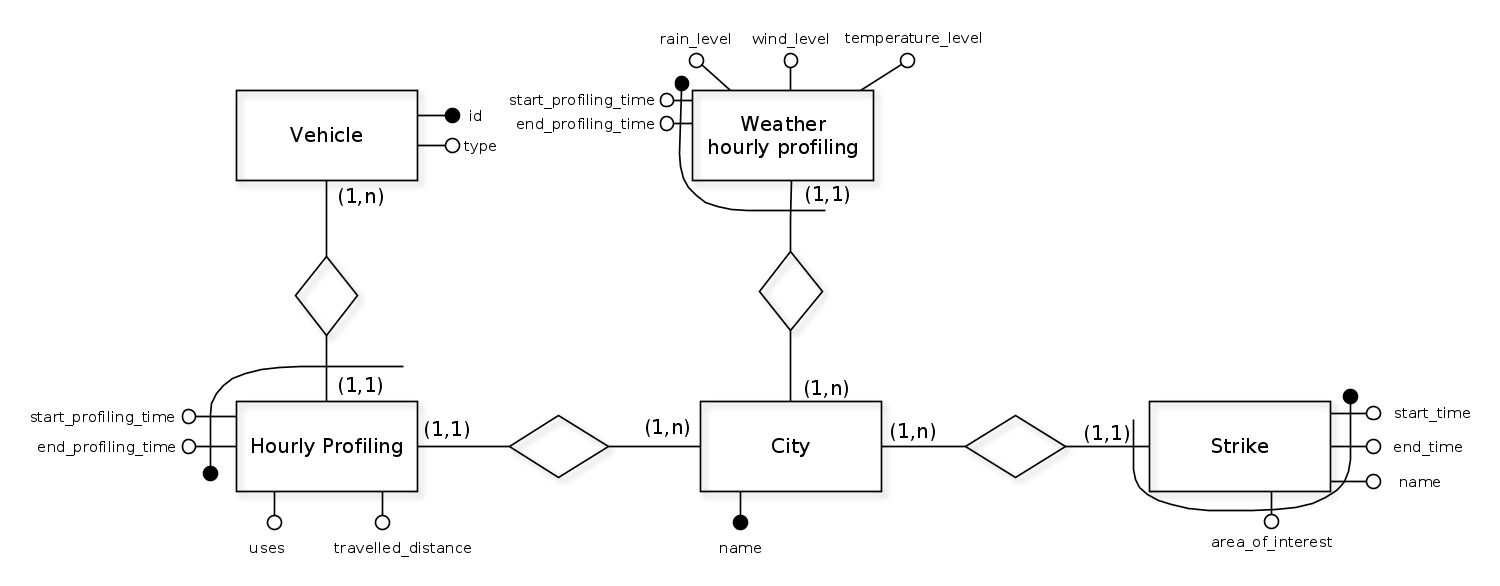
\includegraphics[width=\textwidth]{diagrams/integrated_1_er}                                                                                                                                   
\caption{Diagramma ER Vehicle-Profiling window-Region}                                                                                                                                            
\label{fig:integrated_1_er}                                                                                                                                                           
\end{figure}


